\documentclass{beamer}
\usepackage[utf8]{inputenc}

\usetheme{Madrid}
\usecolortheme{default}
\usepackage{amsmath,amssymb,amsfonts,amsthm}
\usepackage{txfonts}
\usepackage{tkz-euclide}
\usepackage{listings}
\usepackage{adjustbox}
\usepackage{array}
\usepackage{tabularx}
\usepackage{gvv}
\usepackage{lmodern}
\usepackage{circuitikz}
\usepackage{tikz}
\usepackage{graphicx}
\usepackage{mathtools}
\setbeamertemplate{page number in head/foot}[totalframenumber]

\usepackage{tcolorbox}
\tcbuselibrary{minted,breakable,xparse,skins}



\definecolor{bg}{gray}{0.95}
\DeclareTCBListing{mintedbox}{O{}m!O{}}{%
  breakable=true,
  listing engine=minted,
  listing only,
  minted language=#2,
  minted style=default,
  minted options={%
    linenos,
    gobble=0,
    breaklines=true,
    breakafter=,,
    fontsize=\small,
    numbersep=8pt,
    #1},
  boxsep=0pt,
  left skip=0pt,
  right skip=0pt,
  left=25pt,
  right=0pt,
  top=3pt,
  bottom=3pt,
  arc=5pt,
  leftrule=0pt,
  rightrule=0pt,
  bottomrule=2pt,
  toprule=2pt,
  colback=bg,
  colframe=orange!70,
  enhanced,
  overlay={%
    \begin{tcbclipinterior}
    \fill[orange!20!white] (frame.south west) rectangle ([xshift=20pt]frame.north west);
    \end{tcbclipinterior}},
  #3,
}
\lstset{
    language=C,
    basicstyle=\ttfamily\small,
    keywordstyle=\color{blue},
    stringstyle=\color{orange},
    commentstyle=\color{green!60!black},
    numbers=left,
    numberstyle=\tiny\color{gray},
    breaklines=true,
    showstringspaces=false,
}

\title 
{1.10.30}
\date{August 26, 2025}


\author 
{Vivek K Kumar - EE25BTECH11062}



\begin{document}


\frame{\titlepage}
\begin{frame}{Question}
The direction cosines of the vector \myvec{2 \\ 2 \\ -1} are \underline{\hspace{0.1\columnwidth}}
\end{frame}



\begin{frame}{Variables used}
\begin{table}[H]    
  \centering
  

  \caption{Variables Used}
  \label{tab:1.10.30}
\end{table}

\end{frame}

\begin{frame}{Solution}

The unit vector along the direction of given vector is\\
\begin{align}
\frac{A}{\norm{A}} &= \frac{1}{3}\myvec{2 \\ 2 \\ -1} \\
 &=\myvec{\frac{2}{3} \\ \frac{2}{3} \\ \frac{-1}{3}}
\end{align}

\end{frame}

\begin{frame}[fragile]
    \frametitle{Python - Importing libraries and checking system}
    \begin{lstlisting}
import sys
import numpy as np
import numpy.linalg as LA
import matplotlib.pyplot as plt
import matplotlib.image as mpimg

from libs.line.funcs import *
from libs.triangle.funcs import *
from libs.conics.funcs import circ_gen

import subprocess
import shlex

print('Using termux?(y/n)')
y = input()
\end{lstlisting}
\end{frame}

\begin{frame}[fragile]
    \frametitle{Python - Finding direction cosines}
    \begin{lstlisting}
R = np.array([2, 2, -1]).reshape(-1, 1)
O = np.zeros(3).reshape(-1, 1)
norm_R = LA.norm(R)
X = R/norm_R
print(f"The direction cosines of the given vector is \n{X}")
\end{lstlisting}
\end{frame}

\begin{frame}[fragile]
    \frametitle{Python - Generating points and plotting}
    \begin{lstlisting}
p_OR = line_gen(O, R)
p_OX = line_gen(O, X)

fig = plt.figure()
ax = fig.add_subplot(111, projection = '3d')

ax.plot(p_OR[0, :], p_OR[1, :], p_OR[2, :], label = 'Line through OR')
ax.plot(p_OX[0, :], p_OX[1, :], p_OX[2, :], label = 'Direction cosines of OR')
\end{lstlisting}
\end{frame}

\begin{frame}[fragile]
    \frametitle{Python - Labelling points}
    \begin{lstlisting}
line_coords = np.block([[O, R, X]])
ax.scatter(line_coords[0,:], line_coords[1,:], line_coords[2, :])
vert_labels = ['O','R','X']
for i, txt in enumerate(vert_labels):
    ax.text(line_coords[0][i], line_coords[1][i], line_coords[2][i], txt, color='red')

ax.set_xlabel('$x$')
ax.set_ylabel('$y$')
ax.set_zlabel('$z$')
ax.legend(loc='best')
ax.grid(True) 
ax.axis('equal')
    \end{lstlisting}
\end{frame}

\begin{frame}[fragile]
    \frametitle{Python - Saving figure and opening it}
    \begin{lstlisting}
fig.savefig('../figs/fig.png')
print('Saved figure to ../figs/fig.png')

if(y == 'y'):
    subprocess.run(shlex.split('termux-open ../figs/fig.png'))
else:
    subprocess.run(["open",  "../figs/fig.png"])
    \end{lstlisting}
\end{frame}


\begin{frame}{Plot-Using only Python}
    \centering
    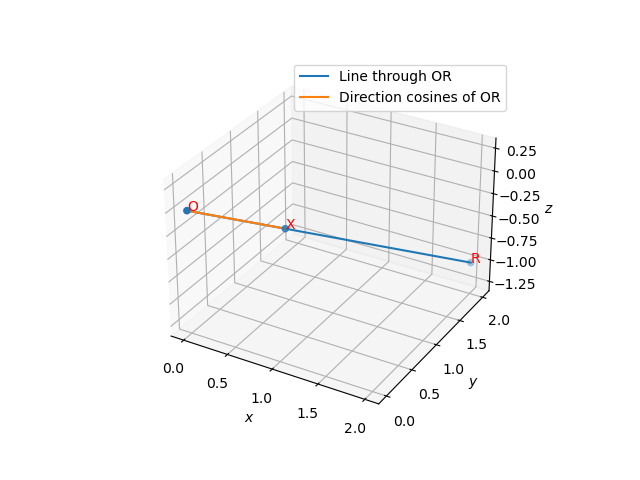
\includegraphics[width=\columnwidth, height=0.8\textheight, keepaspectratio]{../figs/fig.png}     
\end{frame}

\begin{frame}[fragile]
    \frametitle{C Code (0) - Importing libraries}

    \begin{lstlisting}
#include <stdio.h>
#include <stdlib.h>
#include <string.h>
#include <math.h>
#include <sys/socket.h>
#include <netinet/in.h>
#include <unistd.h>
#include "libs/matfun.h"
#include "libs/geofun.h"
    \end{lstlisting}
\end{frame}
\begin{frame}[fragile]
    \frametitle{C Code (1) - Function to Generate Points on a Line}

    \begin{lstlisting}

void point_gen(FILE *p_file, double **A, double **B, int rows, int cols, int npts){
    for(int i = 0; i <= npts; i++){
     double **output = Matadd(A, Matscale(Matsub(B, A, rows, cols), rows, cols, (double)i/npts), rows, cols);
     fprintf(p_file, "%lf, %lf, %lf\n", output[0][0], output[1][0], output[2][0]);
     freeMat(output, rows);
    }
}

    \end{lstlisting}
\end{frame}


\begin{frame}[fragile]
    \frametitle{C Code (2) - Function to write points b/w given point and origin to a file}

    \begin{lstlisting}

void calculate_unit(double **R, int npts);

void write_points(double x1, double y1, double z1, int npts){
    int m = 3;
    int n = 1;

    double **R = createMat(m, n);
    double **O = createMat(m, n);

    R[0][0] = x1;
    R[1][0] = y1;
    R[2][0] = z1;

    O[0][0] = 0;
    O[1][0] = 0;
    O[2][0] = 0;
    \end{lstlisting}
\end{frame}
\begin{frame}[fragile]
    \frametitle{C Code (2) - Function to write points b/w given point and origin to a file}

    \begin{lstlisting}
    FILE *p_file;
    p_file = fopen("plot.dat", "w");
    if(p_file == NULL){
        printf("Error opening data file\n");
    }

    point_gen(p_file, O, R, m, n, npts);
    calculate_unit(R, npts);

    freeMat(R, m);
    freeMat(O, m);

    fclose(p_file);
}

    \end{lstlisting}
\end{frame}

\begin{frame}[fragile]
    \frametitle{C Code (3) - Finding unit vector}

    \begin{lstlisting}

void calculate_unit(double **R, int npts){
    double **X = Matunit(R, 3);
    double **O = createMat(3, 1);

    for(int i = 0; i<3; i++){
        O[i][0] = 0;
    }

    FILE *p_file;
    p_file = fopen("plot2.dat", "w");
    if(p_file == NULL){
        printf("Error opening data file\n");
    }

    point_gen(p_file, O, X, 3, 1, npts);

    \end{lstlisting}
\end{frame}


\begin{frame}[fragile]
    \frametitle{C Code (3) - Finding unit vector}

    \begin{lstlisting}
    freeMat(X, 3);
    freeMat(O, 3);

    fclose(p_file);
}
\end{lstlisting}
\end{frame}

\begin{frame}[fragile]
    \frametitle{Python Code (0) - Importing libraries and checking system}
    \begin{lstlisting}
import numpy as np
import matplotlib.pyplot as plt
import ctypes
import os
import sys
import subprocess

print('Using termux? (y/n)')
termux = input()
\end{lstlisting}
\end{frame}

\begin{frame}[fragile]
    \frametitle{Python Code (1) - Using Shared Object}
    \begin{lstlisting}
lib_path = os.path.join(os.path.dirname(__file__), 'plot.so')
my_lib = ctypes.CDLL(lib_path)

my_lib.write_points.argtypes = [ctypes.c_double, ctypes.c_double, ctypes.c_double, ctypes.c_int]
my_lib.write_points.restype = None
my_lib.write_points(2, 2, -1, 20000)
\end{lstlisting}
\end{frame}

\begin{frame}[fragile]
    \frametitle{Python Code (2) - Loading points and finding unit vector}
    \begin{lstlisting}
points = np.loadtxt('plot.dat', delimiter=',', usecols = (0,1, 2))
points2 = np.loadtxt('plot2.dat', delimiter=',', usecols = (0,1, 2))

x = points[:, 0]
y = points[:, 1]
z = points[:, 2]

x2 = points2[:, 0]
y2 = points2[:, 1]
z2 = points2[:, 2]

print(f"The directions cosines of OR are \n {np.array([x2[-1], y2[-1], z2[-1]]).reshape(-1, 1)}")
\end{lstlisting}
\end{frame}

\begin{frame}[fragile]
    \frametitle{Python Code (3) - Plotting points}
    \begin{lstlisting}
fig = plt.figure()
ax = fig.add_subplot(111, projection = '3d')
ax.plot(x, y, z, label = 'Line through OR')
ax.plot(x2, y2, z2, label = 'Direction cosines of OR')

ax.set_xlabel('$x$')
ax.set_ylabel('$y$')
ax.set_zlabel('$z$')
ax.legend(loc='best')
ax.grid() 
ax.axis('equal')
\end{lstlisting}
\end{frame}

\begin{frame}[fragile]
    \frametitle{Python Code (4) - Labelling points}
    \begin{lstlisting}
line_coords = np.array([[x[0], y[0], z[0]], [x[-1], y[-1], z[-1]], [x2[-1], y2[-1], z2[-1]]])

ax.scatter(line_coords[:, 0], line_coords[:, 1], line_coords[:, 2])
vert_labels = ['O','R','X']
for i, txt in enumerate(vert_labels):
    ax.text(line_coords[i][0], line_coords[i][1], line_coords[i][2], txt, color='red')
\end{lstlisting}    
\end{frame}

\begin{frame}[fragile]
    \frametitle{Python Code (5) - Saving plot and opening it}
    \begin{lstlisting}
fig.savefig('../figs/fig2.png')
print('Saved figure to ../figs/fig2.png')

if(termux == 'y'):
    subprocess.run(shlex.split('termux-open ../figs/fig2.png'))
else:
    subprocess.run(["open",  "../figs/fig2.png"])
\end{lstlisting}
\end{frame}

\begin{frame}{Plot-Using Both C and Python}
    \centering
    
\includegraphics[width=\columnwidth, height=0.8\textheight, keepaspectratio]{../figs/fig2.png}     
\end{frame}

\end{document}
